%%
% Copyright (c) 2017 - 2019, Pascal Wagler;  
% Copyright (c) 2014 - 2019, John MacFarlane
% 
% All rights reserved.
% 
% Redistribution and use in source and binary forms, with or without 
% modification, are permitted provided that the following conditions 
% are met:
% 
% - Redistributions of source code must retain the above copyright 
% notice, this list of conditions and the following disclaimer.
% 
% - Redistributions in binary form must reproduce the above copyright 
% notice, this list of conditions and the following disclaimer in the 
% documentation and/or other materials provided with the distribution.
% 
% - Neither the name of John MacFarlane nor the names of other 
% contributors may be used to endorse or promote products derived 
% from this software without specific prior written permission.
% 
% THIS SOFTWARE IS PROVIDED BY THE COPYRIGHT HOLDERS AND CONTRIBUTORS 
% "AS IS" AND ANY EXPRESS OR IMPLIED WARRANTIES, INCLUDING, BUT NOT 
% LIMITED TO, THE IMPLIED WARRANTIES OF MERCHANTABILITY AND FITNESS 
% FOR A PARTICULAR PURPOSE ARE DISCLAIMED. IN NO EVENT SHALL THE 
% COPYRIGHT OWNER OR CONTRIBUTORS BE LIABLE FOR ANY DIRECT, INDIRECT, 
% INCIDENTAL, SPECIAL, EXEMPLARY, OR CONSEQUENTIAL DAMAGES (INCLUDING,
% BUT NOT LIMITED TO, PROCUREMENT OF SUBSTITUTE GOODS OR SERVICES; 
% LOSS OF USE, DATA, OR PROFITS; OR BUSINESS INTERRUPTION) HOWEVER 
% CAUSED AND ON ANY THEORY OF LIABILITY, WHETHER IN CONTRACT, STRICT 
% LIABILITY, OR TORT (INCLUDING NEGLIGENCE OR OTHERWISE) ARISING IN 
% ANY WAY OUT OF THE USE OF THIS SOFTWARE, EVEN IF ADVISED OF THE 
% POSSIBILITY OF SUCH DAMAGE.
%%

%%
% This is the Eisvogel pandoc LaTeX template.
%
% For usage information and examples visit the official GitHub page:
% https://github.com/Wandmalfarbe/pandoc-latex-template
%%

\PassOptionsToPackage{unicode=true}{hyperref} % options for packages loaded elsewhere
\PassOptionsToPackage{hyphens}{url}
\PassOptionsToPackage{dvipsnames,svgnames*,x11names*,table}{xcolor}
%
\documentclass[
  10pt,
  english,
  letterpaper,
,tablecaptionabove
]{scrartcl}
\usepackage{lmodern}
\usepackage{setspace}
\setstretch{1.2}
\usepackage{amssymb,amsmath}
\usepackage{ifxetex,ifluatex}
\ifnum 0\ifxetex 1\fi\ifluatex 1\fi=0 % if pdftex
  \usepackage[T1]{fontenc}
  \usepackage[utf8]{inputenc}
  \usepackage{textcomp} % provides euro and other symbols
\else % if luatex or xelatex
  \usepackage{unicode-math}
  \defaultfontfeatures{Scale=MatchLowercase}
  \defaultfontfeatures[\rmfamily]{Ligatures=TeX,Scale=1}
\fi
% use upquote if available, for straight quotes in verbatim environments
\IfFileExists{upquote.sty}{\usepackage{upquote}}{}
\IfFileExists{microtype.sty}{% use microtype if available
  \usepackage[]{microtype}
  \UseMicrotypeSet[protrusion]{basicmath} % disable protrusion for tt fonts
}{}
\makeatletter
\@ifundefined{KOMAClassName}{% if non-KOMA class
  \IfFileExists{parskip.sty}{%
    \usepackage{parskip}
  }{% else
    \setlength{\parindent}{0pt}
    \setlength{\parskip}{6pt plus 2pt minus 1pt}}
}{% if KOMA class
  \KOMAoptions{parskip=half}}
\makeatother
\usepackage{xcolor}
\definecolor{default-linkcolor}{HTML}{A50000}
\definecolor{default-filecolor}{HTML}{A50000}
\definecolor{default-citecolor}{HTML}{4077C0}
\definecolor{default-urlcolor}{HTML}{4077C0}
\IfFileExists{xurl.sty}{\usepackage{xurl}}{} % add URL line breaks if available
\IfFileExists{bookmark.sty}{\usepackage{bookmark}}{\usepackage{hyperref}}
\hypersetup{
  pdftitle={B and B+ Trees},
  pdfauthor={Connor Baker},
  pdfsubject={B and B+ Trees},
  pdfkeywords={Lecture, Trees, B Trees, B+ Trees},
  pdfborder={0 0 0},
  breaklinks=true}
\urlstyle{same}  % don't use monospace font for urls
\usepackage[margin=2.5cm,includehead=true,includefoot=true,centering]{geometry}
\usepackage{listings}
\newcommand{\passthrough}[1]{#1}
\lstset{defaultdialect=[5.3]Lua}
\lstset{defaultdialect=[x86masm]Assembler}
\usepackage{graphicx,grffile}
\makeatletter
\def\maxwidth{\ifdim\Gin@nat@width>\linewidth\linewidth\else\Gin@nat@width\fi}
\def\maxheight{\ifdim\Gin@nat@height>\textheight\textheight\else\Gin@nat@height\fi}
\makeatother
% Scale images if necessary, so that they will not overflow the page
% margins by default, and it is still possible to overwrite the defaults
% using explicit options in \includegraphics[width, height, ...]{}
\setkeys{Gin}{width=\maxwidth,height=\maxheight,keepaspectratio}
\setlength{\emergencystretch}{3em}  % prevent overfull lines
\providecommand{\tightlist}{%
  \setlength{\itemsep}{0pt}\setlength{\parskip}{0pt}}
\setcounter{secnumdepth}{-\maxdimen} % remove section numbering
% Redefines (sub)paragraphs to behave more like sections
\ifx\paragraph\undefined\else
  \let\oldparagraph\paragraph
  \renewcommand{\paragraph}[1]{\oldparagraph{#1}\mbox{}}
\fi
\ifx\subparagraph\undefined\else
  \let\oldsubparagraph\subparagraph
  \renewcommand{\subparagraph}[1]{\oldsubparagraph{#1}\mbox{}}
\fi

% Make use of float-package and set default placement for figures to H
\usepackage{float}
\floatplacement{figure}{H}

\setcounter{page}{0}
\lstset{breaklines=true}
\lstset{postbreak=\raisebox{0ex}[0ex][0ex]{\ensuremath{\color{blue}\hookrightarrow\space}}}
\usepackage{datetime}
\settimeformat{ampmtime}
\usepackage{lastpage}
\ifnum 0\ifxetex 1\fi=0 % if pdftex or luatex
  \usepackage[shorthands=off,main=english]{babel}
\else % if xetex
    % See issue https://github.com/reutenauer/polyglossia/issues/127
  \renewcommand*\familydefault{\sfdefault}
    % load polyglossia as late as possible as it *could* call bidi if RTL lang (e.g. Hebrew or Arabic)
  \usepackage{polyglossia}
  \setmainlanguage[]{english}
\fi

\title{B and B+ Trees}
\usepackage{etoolbox}
\makeatletter
\providecommand{\subtitle}[1]{% add subtitle to \maketitle
  \apptocmd{\@title}{\par {\large #1 \par}}{}{}
}
\makeatother
\subtitle{B and B+ Trees and operations on them}
\author{Connor Baker}
\date{2019-04-30, Compiled on \today~at \currenttime}





%%
%% added
%%

%
% language specification
%
% If no language is specified, use English as the default main document language.
%


%
% for the background color of the title page
%
\usepackage{pagecolor}
\usepackage{afterpage}

%
% TOC depth and 
% section numbering depth
%
\setcounter{tocdepth}{3}

%
% break urls
%
\PassOptionsToPackage{hyphens}{url}

%
% When using babel or polyglossia with biblatex, loading csquotes is recommended 
% to ensure that quoted texts are typeset according to the rules of your main language.
%
\usepackage{csquotes}

%
% captions
%
\definecolor{caption-color}{HTML}{777777}
\usepackage[font={stretch=1.2}, textfont={color=caption-color}, position=top, skip=4mm, labelfont=bf, singlelinecheck=false, justification=raggedright]{caption}
\setcapindent{0em}

%
% blockquote
%
\definecolor{blockquote-border}{RGB}{221,221,221}
\definecolor{blockquote-text}{RGB}{119,119,119}
\usepackage{mdframed}
\newmdenv[rightline=false,bottomline=false,topline=false,linewidth=3pt,linecolor=blockquote-border,skipabove=\parskip]{customblockquote}
\renewenvironment{quote}{\begin{customblockquote}\list{}{\rightmargin=0em\leftmargin=0em}%
\item\relax\color{blockquote-text}\ignorespaces}{\unskip\unskip\endlist\end{customblockquote}}

%
% Source Sans Pro as the de­fault font fam­ily
% Source Code Pro for monospace text
%
% 'default' option sets the default 
% font family to Source Sans Pro, not \sfdefault.
%
\usepackage[default]{sourcesanspro}
\usepackage{sourcecodepro}

% XeLaTeX specific adjustments for straight quotes: https://tex.stackexchange.com/a/354887
% This issue is already fixed (see https://github.com/silkeh/latex-sourcecodepro/pull/5) but the 
% fix is still unreleased.
% TODO: Remove this workaround when the new version of sourcecodepro is released on CTAN.
\ifxetex
\makeatletter
\defaultfontfeatures[\ttfamily]
  { Numbers   = \sourcecodepro@figurestyle,
    Scale     = \SourceCodePro@scale,
    Extension = .otf }
\setmonofont
  [ UprightFont    = *-\sourcecodepro@regstyle,
    ItalicFont     = *-\sourcecodepro@regstyle It,
    BoldFont       = *-\sourcecodepro@boldstyle,
    BoldItalicFont = *-\sourcecodepro@boldstyle It ]
  {SourceCodePro}
\makeatother
\fi

%
% heading color
%
\definecolor{heading-color}{RGB}{40,40,40}
\addtokomafont{section}{\color{heading-color}}
% When using the classes report, scrreprt, book, 
% scrbook or memoir, uncomment the following line.
%\addtokomafont{chapter}{\color{heading-color}}

%
% variables for title and author
%
\usepackage{titling}
\title{B and B+ Trees}
\author{Connor Baker}

%
% tables
%

%
% remove paragraph indention
%
\setlength{\parindent}{0pt}
\setlength{\parskip}{6pt plus 2pt minus 1pt}
\setlength{\emergencystretch}{3em}  % prevent overfull lines

%
%
% Listings
%
%


%
% listing colors
%
\definecolor{listing-background}{HTML}{F7F7F7}
\definecolor{listing-rule}{HTML}{B3B2B3}
\definecolor{listing-numbers}{HTML}{B3B2B3}
\definecolor{listing-text-color}{HTML}{000000}
\definecolor{listing-keyword}{HTML}{435489}
\definecolor{listing-identifier}{HTML}{435489}
\definecolor{listing-string}{HTML}{00999A}
\definecolor{listing-comment}{HTML}{8E8E8E}
\definecolor{listing-javadoc-comment}{HTML}{006CA9}

\lstdefinestyle{eisvogel_listing_style}{
  language         = java,
  numbers          = left,
  xleftmargin      = 2.7em,
  framexleftmargin = 2.5em,
  backgroundcolor  = \color{listing-background},
  basicstyle       = \color{listing-text-color}\small\ttfamily{}\linespread{1.15}, % print whole listing small
  breaklines       = true,
  frame            = single,
  framesep         = 0.19em,
  rulecolor        = \color{listing-rule},
  frameround       = ffff,
  tabsize          = 4,
  numberstyle      = \color{listing-numbers},
  aboveskip        = -0.7em,
  belowskip        = 0.1em,
  abovecaptionskip = 0em,
  belowcaptionskip = 1em,
  keywordstyle     = \color{listing-keyword}\bfseries,
  classoffset      = 0,
  sensitive        = true,
  identifierstyle  = \color{listing-identifier},
  commentstyle     = \color{listing-comment},
  morecomment      = [s][\color{listing-javadoc-comment}]{/**}{*/},
  stringstyle      = \color{listing-string},
  showstringspaces = false,
  escapeinside     = {/*@}{@*/}, % Allow LaTeX inside these special comments
  literate         =
  {á}{{\'a}}1 {é}{{\'e}}1 {í}{{\'i}}1 {ó}{{\'o}}1 {ú}{{\'u}}1
  {Á}{{\'A}}1 {É}{{\'E}}1 {Í}{{\'I}}1 {Ó}{{\'O}}1 {Ú}{{\'U}}1
  {à}{{\`a}}1 {è}{{\'e}}1 {ì}{{\`i}}1 {ò}{{\`o}}1 {ù}{{\`u}}1
  {À}{{\`A}}1 {È}{{\'E}}1 {Ì}{{\`I}}1 {Ò}{{\`O}}1 {Ù}{{\`U}}1
  {ä}{{\"a}}1 {ë}{{\"e}}1 {ï}{{\"i}}1 {ö}{{\"o}}1 {ü}{{\"u}}1
  {Ä}{{\"A}}1 {Ë}{{\"E}}1 {Ï}{{\"I}}1 {Ö}{{\"O}}1 {Ü}{{\"U}}1
  {â}{{\^a}}1 {ê}{{\^e}}1 {î}{{\^i}}1 {ô}{{\^o}}1 {û}{{\^u}}1
  {Â}{{\^A}}1 {Ê}{{\^E}}1 {Î}{{\^I}}1 {Ô}{{\^O}}1 {Û}{{\^U}}1
  {œ}{{\oe}}1 {Œ}{{\OE}}1 {æ}{{\ae}}1 {Æ}{{\AE}}1 {ß}{{\ss}}1
  {ç}{{\c c}}1 {Ç}{{\c C}}1 {ø}{{\o}}1 {å}{{\r a}}1 {Å}{{\r A}}1
  {€}{{\EUR}}1 {£}{{\pounds}}1 {«}{{\guillemotleft}}1
  {»}{{\guillemotright}}1 {ñ}{{\~n}}1 {Ñ}{{\~N}}1 {¿}{{?`}}1
  {…}{{\ldots}}1 {≥}{{>=}}1 {≤}{{<=}}1 {„}{{\glqq}}1 {“}{{\grqq}}1
  {”}{{''}}1
}
\lstset{style=eisvogel_listing_style}

\lstdefinelanguage{XML}{
  morestring      = [b]",
  moredelim       = [s][\bfseries\color{listing-keyword}]{<}{\ },
  moredelim       = [s][\bfseries\color{listing-keyword}]{</}{>},
  moredelim       = [l][\bfseries\color{listing-keyword}]{/>},
  moredelim       = [l][\bfseries\color{listing-keyword}]{>},
  morecomment     = [s]{<?}{?>},
  morecomment     = [s]{<!--}{-->},
  commentstyle    = \color{listing-comment},
  stringstyle     = \color{listing-string},
  identifierstyle = \color{listing-identifier}
}

%
% header and footer
%
\usepackage{fancyhdr}

\fancypagestyle{eisvogel-header-footer}{
  \fancyhead{}
  \fancyfoot{}
  \lhead[2019-04-30]{B and B+ Trees}
  \chead[]{}
  \rhead[B and B+ Trees]{2019-04-30}
  \lfoot[\thepage~of \pageref{LastPage}]{Connor Baker}
  \cfoot[]{}
  \rfoot[Connor Baker]{\thepage~of \pageref{LastPage}}
  \renewcommand{\headrulewidth}{0.4pt}
  \renewcommand{\footrulewidth}{0.4pt}
}
\pagestyle{eisvogel-header-footer}

%%
%% end added
%%

\begin{document}

%%
%% begin titlepage
%%

\begin{titlepage}
\newgeometry{left=6cm}
\definecolor{titlepage-color}{HTML}{FFFFFF}
\newpagecolor{titlepage-color}\afterpage{\restorepagecolor}
\newcommand{\colorRule}[3][black]{\textcolor[HTML]{#1}{\rule{#2}{#3}}}
\begin{flushleft}
\noindent
\\[-1em]
\color[HTML]{0d47a1}
\makebox[0pt][l]{\colorRule[0d47a1]{1.3\textwidth}{2pt}}
\par
\noindent

{ \setstretch{1.4}
\vfill
\noindent {\huge \textbf{\textsf{B and B+ Trees}}}
\vskip 1em
{\Large \textsf{B and B+ Trees and operations on them}}
\vskip 2em
\noindent
{\Large \textsf{Connor Baker}
\vfill
}


\textsf{2019-04-30, Compiled on \today~at \currenttime}}
\end{flushleft}
\end{titlepage}
\restoregeometry

%%
%% end titlepage
%%



\hypertarget{b-and-b-trees}{%
\section{B and B+ Trees}\label{b-and-b-trees}}

\hypertarget{review-binary-search-trees}{%
\subsection{Review: Binary Search
Trees}\label{review-binary-search-trees}}

\begin{itemize}
\tightlist
\item
  Stores a collection of sorted values

  \begin{itemize}
  \tightlist
  \item
    The left subtree is less than the parent which is less than the
    right subtree
  \item
    There are no duplicates allowed
  \end{itemize}
\item
  Basic operations

  \begin{itemize}
  \tightlist
  \item
    Searching through the tree, inserting into the tree, and removing
    items from the tree
  \item
    All operate in \(O(\)height\()\) of the tree
  \end{itemize}
\item
  Balanced tree variations

  \begin{itemize}
  \tightlist
  \item
    AVL and Red-Black trees
  \item
    Operates in \(O(\log_2(n))\)
  \end{itemize}
\end{itemize}

\hypertarget{binary-search-trees}{%
\subsection{Binary Search Trees}\label{binary-search-trees}}

\begin{itemize}
\tightlist
\item
  So far we have:

  \begin{itemize}
  \tightlist
  \item
    \(n\) as the number of items to store, which is equivalent to the
    number of tree nodes
  \item
    The tree height (if it's balanced) is usually about \(\log_2(n)\)
  \end{itemize}
\item
  How can we improve on this?

  \begin{itemize}
  \tightlist
  \item
    We can increase the number of branches: let every node have \(c\)
    child noes. The new tree height would be about \(\log_c(n)\)
  \item
    Combine multiple nodes into one: a single node represents \(m\)
    items. The new tree's size would be \(\frac{n}{m}\)
  \item
    This in particular is especially helpful when data doesn't fit in
    memory

    \begin{itemize}
    \tightlist
    \item
      Dis access is much slower than memory access
    \item
      Breaking up items into size-\(m\) groups to transfer from disk to
      memory is much more efficient
    \end{itemize}
  \end{itemize}
\end{itemize}

\hypertarget{b-trees-and-variations}{%
\subsection{B-Trees and Variations}\label{b-trees-and-variations}}

\begin{itemize}
\tightlist
\item
  Commonly used in databases and file systems

  \begin{itemize}
  \tightlist
  \item
    They were invented by Rudolf Bayer and Ed McCreight while working at
    Boeing Research Labs in 1972
  \item
    B could stand for: Balanced, Broad, Bushy, Boeing, or Bayer
  \end{itemize}
\item
  2-3 trees

  \begin{itemize}
  \tightlist
  \item
    Every non-leaf node has either two or three children
  \item
    Restricted, simpler version of B-Trees
  \end{itemize}
\item
  B+ Trees

  \begin{itemize}
  \tightlist
  \item
    B trees with internal nodes not storing data -- they only store keys
  \item
    Weiss 19.8 presents B+ trees, if you'd like additional reading
  \end{itemize}
\item
  B\(^*\) Trees

  \begin{itemize}
  \tightlist
  \item
    B+ trees where every non-leaf node is at least \(\frac{2}{3}\) full
  \end{itemize}
\end{itemize}

\hypertarget{trees}{%
\subsection{2-3 Trees}\label{trees}}

\begin{itemize}
\tightlist
\item
  Every node has between two and three children

  \begin{itemize}
  \tightlist
  \item
    Nodes are described by the number of children they have

    \begin{itemize}
    \tightlist
    \item
      A 2-node has two children and a 3-node has three children
    \end{itemize}
  \end{itemize}
\item
  Every node has between one and two values

  \begin{itemize}
  \tightlist
  \item
    A non-leaf node with \(m\) values must have \(m+1\) children
  \end{itemize}
\item
  Generalized ordering rules between values and subtrees

  \begin{itemize}
  \tightlist
  \item
    Similar to how we did with BSTs
  \item
    There are also no duplicate values allowed, again, similar to BSTs
  \end{itemize}
\end{itemize}

\hypertarget{ordering-examples}{%
\subsection{Ordering Examples}\label{ordering-examples}}

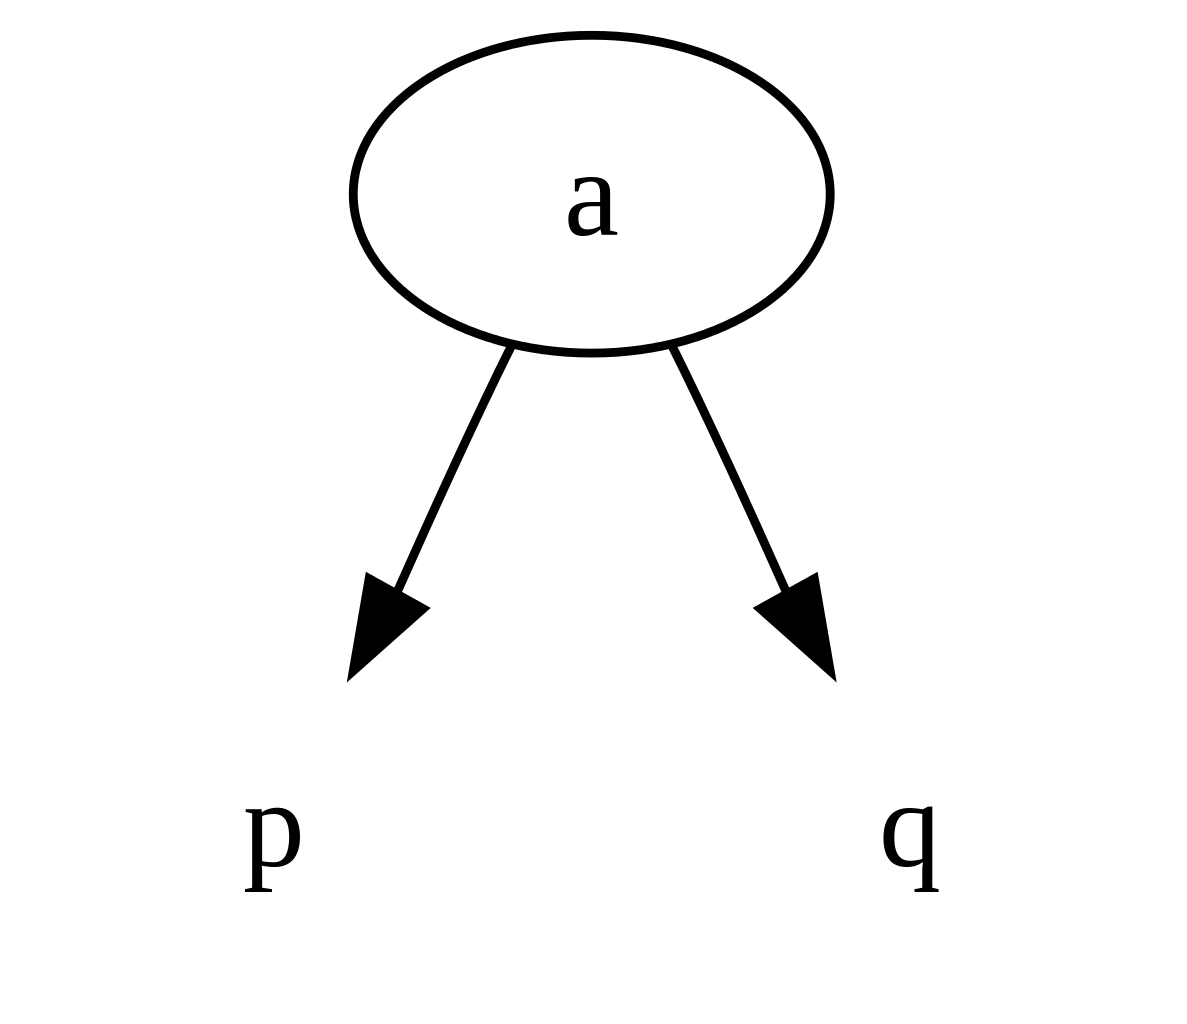
\includegraphics[width=0.25\textwidth,height=\textheight]{images/1.png}
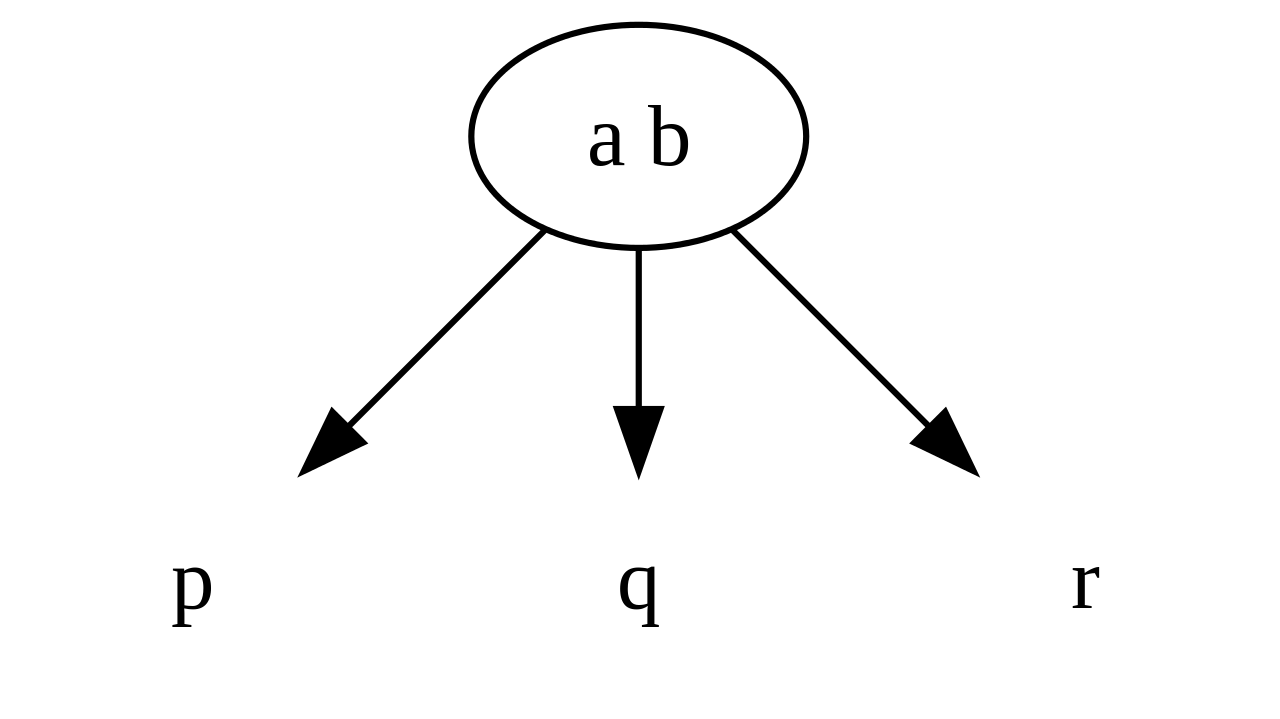
\includegraphics[width=0.4\textwidth,height=\textheight]{images/2.png}

\begin{itemize}
\tightlist
\item
  2-node

  \begin{itemize}
  \tightlist
  \item
    1 value (which is \(a\)) and 2 subtrees (\(p\) and \(q\))
  \item
    \(p < a < q\)
  \end{itemize}
\item
  3-node

  \begin{itemize}
  \tightlist
  \item
    2 values (\(a\) and \(b\)) and 3 subtrees (\(p,q\) and \(r\))
  \item
    \(p < a < q < b < r\)
  \end{itemize}
\end{itemize}

\hypertarget{tree-operations}{%
\subsection{2-3 Tree Operations}\label{tree-operations}}

\begin{itemize}
\tightlist
\item
  Search: similar to BSTs
\item
  Insertion: when inserting a new value, the tree grows
  \enquote{upwards}

  \begin{itemize}
  \tightlist
  \item
    Walk down to add the value into a leaf
  \item
    If the node is too big split it and promote the median to a higher
    level

    \begin{itemize}
    \tightlist
    \item
      This could in turn cause a sequence of splitting
    \end{itemize}
  \end{itemize}
\item
  Deletion: many possible cases

  \begin{itemize}
  \tightlist
  \item
    Shrinking, merging, and shifting
  \end{itemize}
\end{itemize}

\hypertarget{b-trees}{%
\subsection{B-Trees}\label{b-trees}}

\begin{itemize}
\tightlist
\item
  A B-Tree is a search tree

  \begin{itemize}
  \tightlist
  \item
    It uses a generalized ordering property
  \end{itemize}
\item
  A B-Tree of order \(m\) requires that for each non-leaf node

  \begin{itemize}
  \tightlist
  \item
    The number of children is between \(\frac{m}{2}\) and \(m\)

    \begin{itemize}
    \tightlist
    \item
      Exception: the root has at least two children and is not a leaf
    \end{itemize}
  \item
    The number of values is between \(frac{m}{2} - 1\) and \(m - 1\)
  \end{itemize}
\item
  The number of values in a leaf node is bounded above by \(\ell\)
\item
  Every path from the root to a leaf in a B-tree must have the same
  length
\item
  \emph{Note}: a 2-3 tree is a B-tree with \(m=3\) and \(\ell=2\)
\end{itemize}

\hypertarget{b-trees-vs.-bsts}{%
\subsection{B-Trees vs.~BSTs}\label{b-trees-vs.-bsts}}

\begin{figure}
\centering
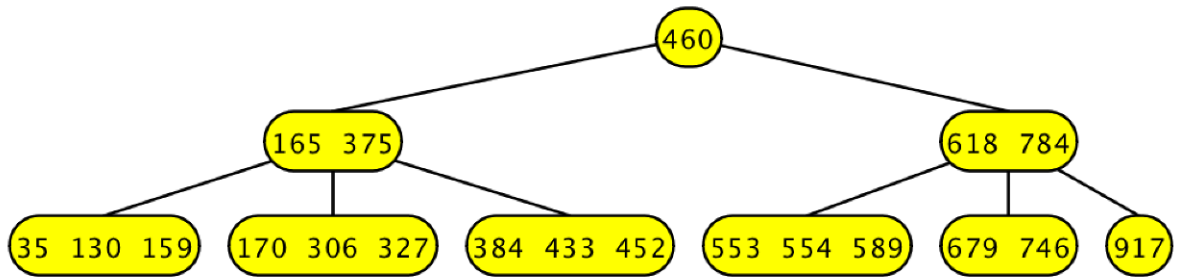
\includegraphics[width=0.75\textwidth,height=\textheight]{images/3.png}
\caption{A B-Tree}
\end{figure}

\begin{itemize}
\tightlist
\item
  Comparison with BSTs

  \begin{itemize}
  \tightlist
  \item
    They're both search trees, and they're both balanced
  \item
    The smaller height is caused by larger nodes -- this is typically
    more memory friendly, and B-Trees provide us with the flexibility to
    tune \(m\) and \(\ell\) values based on memory configuration
  \end{itemize}
\item
  Operations are similar to 2-3 trees
\end{itemize}

\hypertarget{b-trees-1}{%
\subsection{B+ Trees}\label{b-trees-1}}

\begin{itemize}
\tightlist
\item
  B-Trees in which the nodes store only keys, not data
\item
  We use those keys to guide the direction of our searches when walking
  down the tree
\item
  All values are stored in leaves

  \begin{itemize}
  \tightlist
  \item
    It's like a tree and an array combined
  \end{itemize}
\end{itemize}

\hypertarget{b-tree-example}{%
\subsection{B+ Tree Example}\label{b-tree-example}}

\begin{figure}
\centering
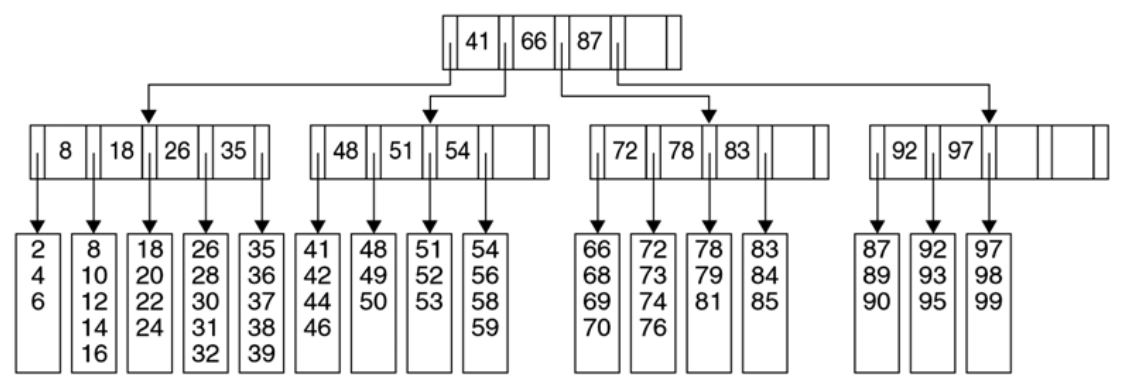
\includegraphics[width=0.75\textwidth,height=\textheight]{images/4.png}
\caption{An example B+-Tree with \(m=\ell=5\)}
\end{figure}

\begin{itemize}
\tightlist
\item
  All non-leaf nodes have between 3 and 5 children

  \begin{itemize}
  \tightlist
  \item
    Which also means that the number of keys is bounded by 2 and 4
  \end{itemize}
\item
  Each leaf node has between 3 and 5 dta items

  \begin{itemize}
  \tightlist
  \item
    \(\lceil \frac{\ell}{2} \rceil \leq\) number of data items
    \(\leq \ell\)
  \end{itemize}
\item
  \emph{Note}: \(m\) and \(\ell\) can be different values
\end{itemize}

\hypertarget{operations-on-b-trees}{%
\subsection{Operations on B+-Trees}\label{operations-on-b-trees}}

\begin{itemize}
\tightlist
\item
  Search: similar to BSTs

  \begin{itemize}
  \tightlist
  \item
    Use a group of keys to pick from a group of links to continue
    searching
  \end{itemize}
\item
  Insertion: adding a value into a leaf

  \begin{itemize}
  \tightlist
  \item
    If the leaf isn't full expand the node and insert the keys
  \item
    If the leaf would become full, split the node in two

    \begin{itemize}
    \tightlist
    \item
      This triggers a recursive process, and we may have to go all the
      way to the root, splitting than, and add one level to every path
    \end{itemize}
  \end{itemize}
\item
  Deletion: removing a value from a leaf

  \begin{itemize}
  \tightlist
  \item
    Remove the value
  \item
    If the node gets too small, we need to merge/adjust with a sibling
  \item
    Similarly, we may need to go all the way to the root and reduce the
    height of the tree
  \end{itemize}
\end{itemize}

\hypertarget{b-tree-search-examples}{%
\subsection{B+-Tree Search Examples}\label{b-tree-search-examples}}

Suppose we have the following tree

\begin{figure}
\centering
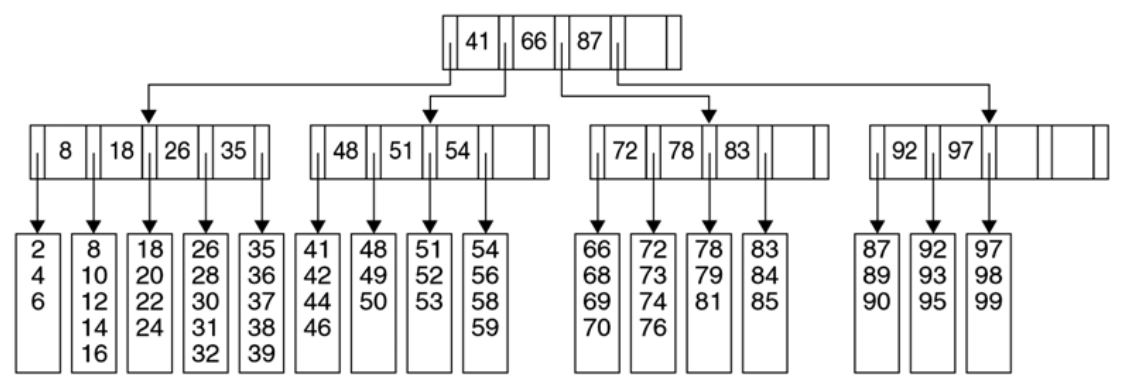
\includegraphics[width=0.75\textwidth,height=\textheight]{images/4.png}
\caption{An example B+-Tree with \(m=\ell=5\)}
\end{figure}

and we want to search for the value \passthrough{\lstinline!31!}. Search
proceeds in much the same way that it does in an equivalent BST:

\begin{figure}
\centering
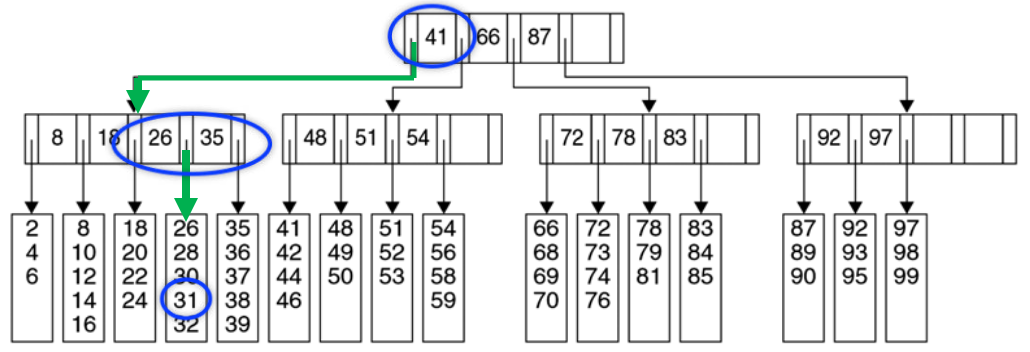
\includegraphics[width=0.75\textwidth,height=\textheight]{images/5.png}
\caption{Tracing the search for \passthrough{\lstinline!31!} through a
B+-Tree with \(m=\ell=5\)}
\end{figure}

\begin{itemize}
\tightlist
\item
  \passthrough{\lstinline!31 < 41!}, take the leftmost tree
\item
  \passthrough{\lstinline!26 < 31 < 35!}, take the tree which is second
  from the right
\item
  \passthrough{\lstinline!31!} is in the array, so we've found it
\end{itemize}

Suppose now that we want to find \passthrough{\lstinline!57!}.

\begin{figure}
\centering
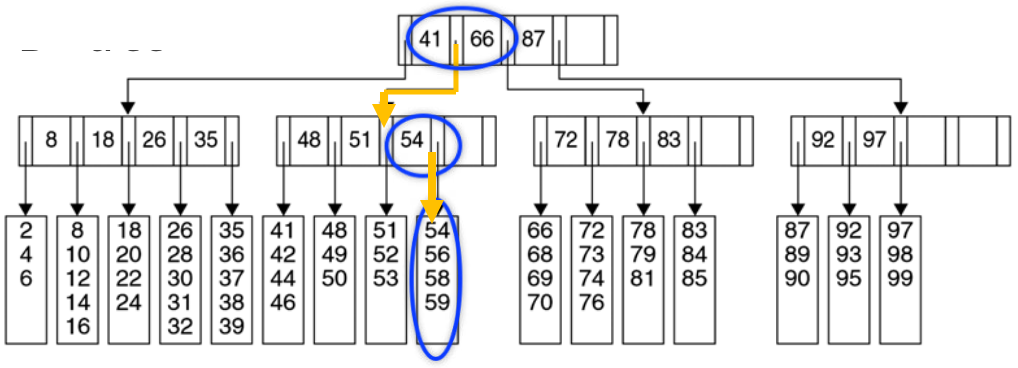
\includegraphics[width=0.75\textwidth,height=\textheight]{images/6.png}
\caption{Tracing the search for \passthrough{\lstinline!57!} through a
B+-Tree with \(m=\ell=5\)}
\end{figure}

\begin{itemize}
\tightlist
\item
  \passthrough{\lstinline!41 < 57 < 66!}, take the tree second to the
  left
\item
  \passthrough{\lstinline!54 < 57!}, take the rightmost tree available
\item
  \passthrough{\lstinline!57!} isn't in the array, so it must not be in
  the tree
\end{itemize}

\hypertarget{b-tree-insertion-examples}{%
\subsection{B+-Tree Insertion
Examples}\label{b-tree-insertion-examples}}

Suppose that we want to insert \passthrough{\lstinline!57!} into the
B+-Tree from the previous example. We first find the array in which we
will insert \passthrough{\lstinline!57!}:

\begin{figure}
\centering
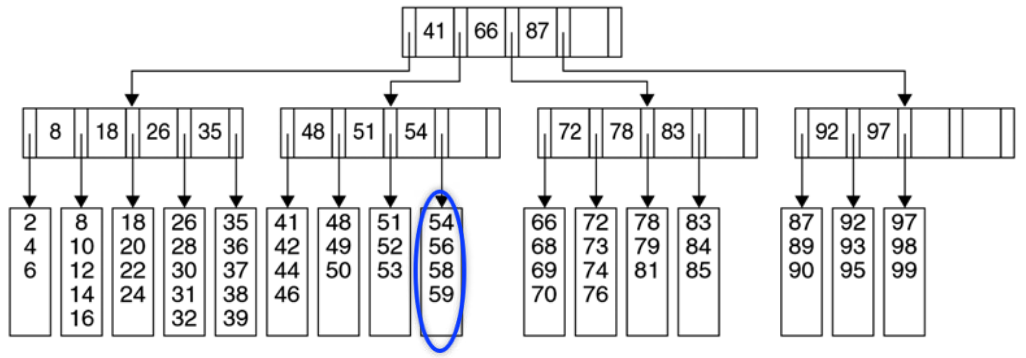
\includegraphics[width=0.75\textwidth,height=\textheight]{images/7.png}
\caption{Finding the array into which we will insert
\passthrough{\lstinline!57!}}
\end{figure}

Inserting \passthrough{\lstinline!57!} is as simple as adding it to the
array.

\begin{figure}
\centering
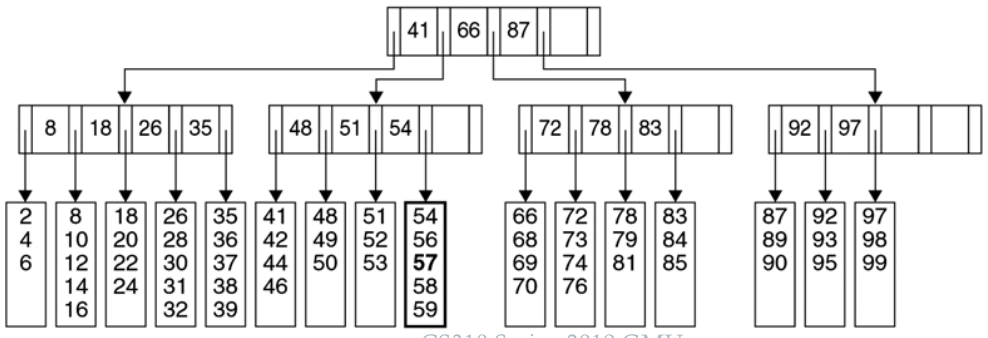
\includegraphics[width=0.75\textwidth,height=\textheight]{images/8.png}
\caption{After inserting \passthrough{\lstinline!57!} into the array}
\end{figure}

However, upon a subsequent insertion of a value which would also go into
that array, like \passthrough{\lstinline!55!}, we're forced to split the
array and add a node to the second half, like so:

\begin{figure}
\centering
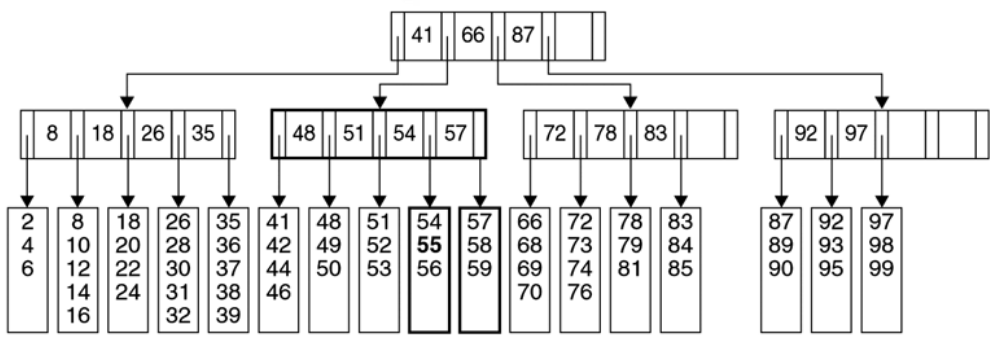
\includegraphics[width=0.75\textwidth,height=\textheight]{images/9.png}
\caption{After inserting \passthrough{\lstinline!55!} into the B+-Tree}
\end{figure}

It's possible that, unlike with the previous example, we don't have room
to add a node. In that case, we split the parent.

Consider what happens when we try to add \passthrough{\lstinline!40!}
into the tree.

\begin{figure}
\centering
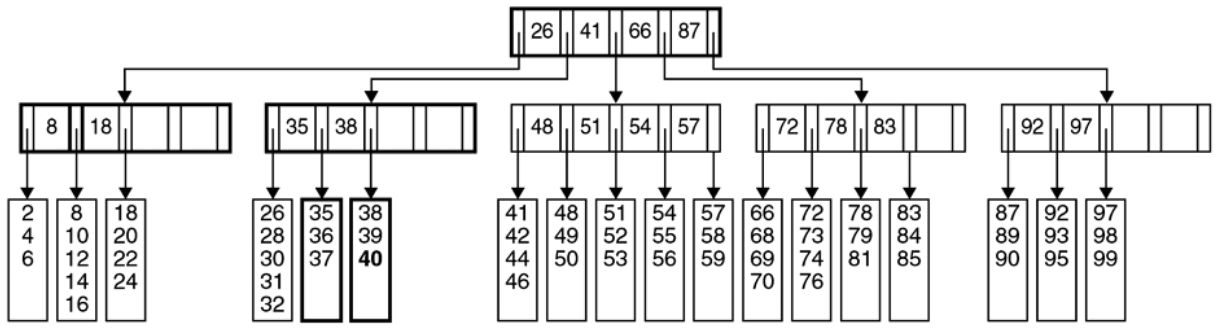
\includegraphics[width=0.85\textwidth,height=\textheight]{images/10.png}
\caption{After inserting \passthrough{\lstinline!40!} into the B+-Tree}
\end{figure}

The array is already full, so we split the array into equal parts
(\([35,37]\) and \([38,40]\)). However, there's no place to put the
split array, so we have to split the parent.

We push \passthrough{\lstinline!26!} up into the root, and split the
parent into two pieces: the first array contains
\passthrough{\lstinline!8!} and \passthrough{\lstinline!18!}, and the
second array contains \passthrough{\lstinline!35!} and
\passthrough{\lstinline!38!}. A valid question at this point is
\enquote{where did the \passthrough{\lstinline!38!} come from?} Recall
that the values of the parent are the base of the array, and that the
number of values of the parent are always one less than the number of
values in the array. For us to have three arrays attached to the parent,
the parent must hold two keys. To get the additional key (since we only
had \passthrough{\lstinline!35!} originally) we must take the first
value of the array and add that, as a key, to the parent.

Suppose now that we want to delete the value
\passthrough{\lstinline!99!} from the tree.

\begin{figure}
\centering
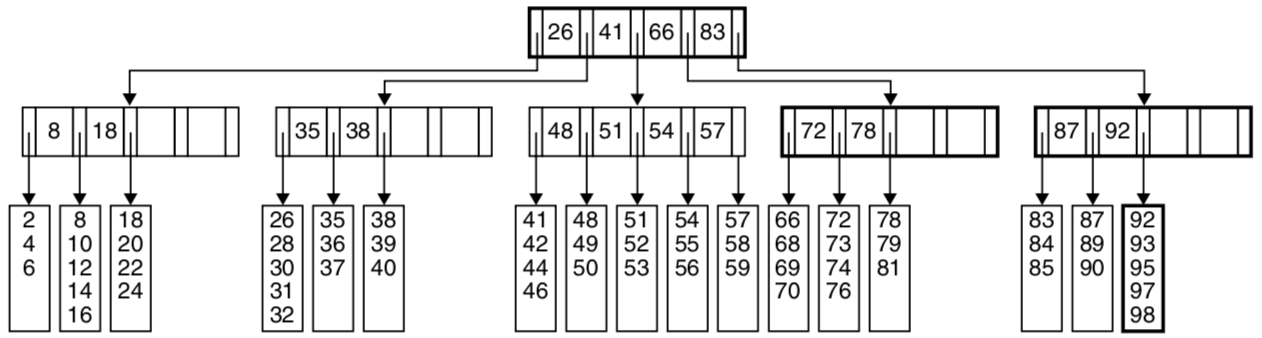
\includegraphics[width=0.85\textwidth,height=\textheight]{images/11.png}
\caption{After deleting \passthrough{\lstinline!99!} from the B+-Tree}
\end{figure}

The resulting leaf only has two values and its neighbor has three (which
is the minimum it is allowed to have). To fix this shortage of values,
we can combine the left neighbor and the current leaf to make a new leaf
with five values.

However, doing this creates a parent with two children and a single
value (\passthrough{\lstinline!92!} -- since
\passthrough{\lstinline!97!} is no longer the beginning of the array it
is not a key in the parent). To fix \emph{this} problem we can adopt
from a neighbor that has more than enough -- we take the array beginning
with \passthrough{\lstinline!83!} from the left neighbor, which allows
us to make a new value, \passthrough{\lstinline!87!}, giving us two
values and three children.

\hypertarget{operation-ideas}{%
\subsection{Operation Ideas}\label{operation-ideas}}

\hypertarget{addx-bt}{%
\subsubsection{\texorpdfstring{\texttt{add(x,\ bt)}}{add(x, bt)}}\label{addx-bt}}

\begin{lstlisting}[language=Java]
find leaf in bt for x
if (space in leaf) {
  add x to leaf
} else {
    if (parent has room) {
      new leaf
      split data
      add x to leaf
    } else {
      recurse up
      split internal
      new leaves
      split data
      back down to add x
  }
}
\end{lstlisting}

\hypertarget{removex-bt}{%
\subsubsection{\texorpdfstring{\texttt{remove(x,\ bt)}}{remove(x, bt)}}\label{removex-bt}}

\begin{lstlisting}[language=Java]
find leaf with x
remove x
if (leaf < 1/2 full) {
  merge with neighbor leaf
  steal leaves if needed
  recurse up to adjust
}
\end{lstlisting}

\hypertarget{b-trees-summary}{%
\subsection{B-Trees Summary}\label{b-trees-summary}}

What should the take home be?

\begin{itemize}
\tightlist
\item
  Multi-way trees

  \begin{itemize}
  \tightlist
  \item
    If order-\(k\) nodes are all at least \(\frac{1}{2}\) full, we have
    \(O(\log_k(n))\) height
  \end{itemize}
\item
  Hybrids of arrays and trees exist

  \begin{itemize}
  \tightlist
  \item
    They're sensitive to the memory hierarchy
  \item
    They're good for data that doesn't fit in memory

    \begin{itemize}
    \tightlist
    \item
      Like large databases, or file systems
    \end{itemize}
  \end{itemize}
\item
  They are a simple idea but require complex implementations due to the
  number of cases for supported operations
\item
  There are many variations on the idea
\end{itemize}

\end{document}
